%% 11/23/2015
%%%%%%%%%%%%%%%%%%%%%%%%%%%%%%%%%%%%%%%%%%%%%%%%%%%%%%%%%%%%%%%%%%%%%%%%%%%%
% AGUJournalTemplate.tex: this template file is for articles formatted with LaTeX
%
% This file includes commands and instructions
% given in the order necessary to produce a final output that will
% satisfy AGU requirements. 
%
% You may copy this file and give it your
% article name, and enter your text.
%
%%%%%%%%%%%%%%%%%%%%%%%%%%%%%%%%%%%%%%%%%%%%%%%%%%%%%%%%%%%%%%%%%%%%%%%%%%%%
% PLEASE DO NOT USE YOUR OWN MACROS
% DO NOT USE \newcommand, \renewcommand, or \def, etc.
%
% FOR FIGURES, DO NOT USE \psfrag or \subfigure.
% DO NOT USE \psfrag or \subfigure commands.
%%%%%%%%%%%%%%%%%%%%%%%%%%%%%%%%%%%%%%%%%%%%%%%%%%%%%%%%%%%%%%%%%%%%%%%%%%%%
%
% Step 1: Set the \documentclass
%
% There are two options for article format:
%
% 1) PLEASE USE THE DRAFT OPTION TO SUBMIT YOUR PAPERS.
% The draft option produces double spaced output.
% 
% 2) numberline will give you line numbers.

%% To submit your paper:
\documentclass[draft, linenumbers]{agujournal}
%\draftfalse

%% For final version.
% \documentclass{agujournal}

% Now, type in the journal name: \journalname{<Journal Name>}

% ie, \journalname{Journal of Geophysical Research}
%% Choose from this list of Journals:
%
% JGR-Atmospheres
% JGR-Biogeosciences
% JGR-Earth Surface
% JGR-Oceans
% JGR-Planets
% JGR-Solid Earth
% JGR-Space Physics
% Global Biochemical Cycles
% Geophysical Research Letters
% Paleoceanography
% Radio Science
% Reviews of Geophysics
% Tectonics
% Space Weather
% Water Resource Research
% Geochemistry, Geophysics, Geosystems
% Journal of Advances in Modeling Earth Systems (JAMES)
% Earth's Future
% Earth and Space Science
%
%

\journalname{Geophysical Research Letters}


\begin{document}

%% ------------------------------------------------------------------------ %%
%  Title
% 
% (A title should be specific, informative, and brief. Use
% abbreviations only if they are defined in the abstract. Titles that
% start with general keywords then specific terms are optimized in
% searches)
%
%% ------------------------------------------------------------------------ %%

% Example: \title{This is a test title}

\title{Microburst Scale Size Derived from Multiple Bounces of a Microburst Simultaneously Observed with the FIREBIRD-II CubeSats}

%% ------------------------------------------------------------------------ %%
%
%  AUTHORS AND AFFILIATIONS
%
%% ------------------------------------------------------------------------ %%

% Authors are individuals who have significantly contributed to the
% research and preparation of the article. Group authors are allowed, if
% each author in the group is separately identified in an appendix.)

% List authors by first name or initial followed by last name and
% separated by commas. Use \affil{} to number affiliations, and
% \thanks{} for author notes.  
% Additional author notes should be indicated with \thanks{} (for
% example, for current addresses). 

% Example: \authors{A. B. Author\affil{1}\thanks{Current address, Antartica}, B. C. Author\affil{2,3}, and D. E.
% Author\affil{3,4}\thanks{Also funded by Monsanto.}}

\authors{Mykhaylo Shumko\affil{1}, John Sample\affil{1}, Arlo Johnson\affil{1}, Bern Blake\affil{2}, Alex Crew\affil{3}, Harlan Spence\affil{4}, David Klumpar\affil{1}, Oleksiy Agapitov\affil{5}, Matthew Handley\affil{1}}

\affiliation{1}{Department of Physics, Montana State University, Bozeman, Montana, USA}
\affiliation{2}{Space Science Applications Laboratory, The Aerospace Corporation, Los Angeles, California, USA}
\affiliation{3}{The Johns Hopkins University Applied Physics Laboratory LLC, Laurel, Maryland, USA}
\affiliation{4}{Institute for the Study of Earth, Oceans, and Space, University of New Hampshire, Durham, New Hampshire, USA}
\affiliation{5}{Space Sciences Laboratory, UC Berkeley, Berkeley, California, USA}

%% Corresponding Author:
% Corresponding author mailing address and e-mail address:

% (include name and email addresses of the corresponding author.  More
% than one corresponding author is allowed in this LaTeX file and for
% publication; but only one corresponding author is allowed in our
% editorial system.)  

% Example: \correspondingauthor{First and Last Name}{email@address.edu}

\correspondingauthor{Mykhaylo Shumko}{msshumko@gmail.com}

%% Keypoints, final entry on title page.

% Example: 
% \begin{keypoints}
% \item	List up to three key points (at least one is required)
% \item	Key Points summarize the main points and conclusions of the article
% \item	Each must be 100 characters or less with no special characters or punctuation 
% \end{keypoints}

%  List up to three key points (at least one is required)
%  Key Points summarize the main points and conclusions of the article
%  Each must be 100 characters or less with no special characters or punctuation 

\begin{keypoints}
\item The \added{lower bound} lat/lon scale sizes \added{of the microburst} at LEO were $28.8 \pm 0.8$ km and $50.8 \pm 11.4$ km, respectively.
\item Deduced lower bound equatorial scale size is similar to the whistler-mode chorus source scale.
\end{keypoints}

%% ------------------------------------------------------------------------ %%
%
%  ABSTRACT
%
% A good abstract will begin with a short description of the problem
% being addressed, briefly describe the new data or analyses, then
% briefly states the main conclusion(s) and how they are supported and
% uncertainties. 
%% ------------------------------------------------------------------------ %%

%% \begin{abstract} starts the second page 

\begin{abstract}
The FIREBIRD-II CubeSats simultaneously observed a large \added{spatial scale} microburst with multiple bounces on February 2nd, 2015 during a small storm. This is the first such microburst observed by two spacecraft, and it sheds light on its spatial scale sizes and bounce periods.  Its lower bound latitudinal scale size was $ 28.8 \pm 0.8$ km and the longitudinal scale size was $ 50.8 \pm 11.4$  km in low earth orbit. Using the Tsyganenko 1989 magnetic field model, these scale sizes were mapped to the magnetic equator to get the radial and azimuthal scale sizes of at least $504 \pm​ 14$ km and $530 \pm 119$ km, respectively. These lower bound equatorial scale sizes are similar to whistler-mode chorus wave source scale sizes, which supports the hypothesis that microbursts are a product of electron scattering by chorus waves. Lastly, the electron bounce period from the subsequent bounces was calculated and compared to analytical and numerical bounce times to validate numerous magnetic field models.
\end{abstract}
%% ------------------------------------------------------------------------ %%
%
%  TEXT
%
%% ------------------------------------------------------------------------ %%

%%% Suggested section heads:
% \section{Introduction}
% 
% The main text should start with an introduction. Except for short
% manuscripts (such as comments and replies), the text should be divided
% into sections, each with its own heading. 

% Headings should be sentence fragments and do not begin with a
% lowercase letter or number. Examples of good headings are:

% \section{Materials and Methods}
% Here is text on Materials and Methods.
%
% \subsection{A descriptive heading about methods}
% More about Methods.
% 
% \section{Data} (Or section title might be a descriptive heading about data)
% 
% \section{Results} (Or section title might be a descriptive heading about the
% results)
% 
% \section{Conclusions}

\section{Introduction}\label{Intro}
% use \citet for direct references, \citep for indirect.
The dynamics of radiation belt electrons are complex, and are driven by competition between source and loss processes. A few possible loss processes are radial diffusion \citep{Shprits2004}, magnetopause shadowing \citep{Ukhorskiy2006}, and pitch angle \added{and energy} diffusion \citep[e.g.][]{Abel1998_1, Summers1998, Meredith2002, Selesnick2003, Horne2003, Thorne2005} due to \added{scattering of electrons by} plasma waves. \deleted{and Coulomb scattering.} As described in \citep{Millan2007, Thorne2010} and references contained within, there are a variety of waves that cause pitch angle scattering, including electromagnetic ion cyclotron waves, plasmaspheric hiss, and \deleted{whistler-mode} chorus. Whistler-mode chorus predominantly occurs in the dawn sector \citep{Li2009} where it accelerates electrons with large equatorial pitch angles and scatters electrons with small equatorial pitch angles \citep{Horne2003}. Some of these electrons may be impulsively scattered into the loss cone, \replaced{This sudden increase (duration ${\approx} 100$ ms) in precipitating electron flux is believed to be caused by scattering with whistler-mode chorus waves}{where they result in short-duration ($\sim 100$ ms) enhancements in precipitating flux called microbursts.}

\deleted{Microbursts were first termed by} \citet{Anderson1964} \added{coined the term microburst to describe enhancements of} \deleted{who used high altitude balloon observations of} bremsstrahlung X-rays emitted from scattered electrons impacting the atmosphere, \added{observed by high altitude balloons}. Since then, microbursts have routinely been observed with other balloon missions \citep{Parks1967, Woodger2015, Anderson2017}. Relativistic microbursts have not yet been observed by high altitude balloons in the dawn sector \citep{Millan2002, Millan2007}. \replaced{, which may be caused by a pitch angle anisotropy of relativistic microbursts due to relatively weaker pitch angle scattering of relativistic electrons by chorus }{This may be due to relatively weaker pitch angle scattering of relativistic electrons by chorus} \citep{Lee2012}. Microbursts have also been observed in low earth orbit (LEO) with, e.g. the SAMPEX \added{> 150 keV} and > 1 MeV channels \citep{Nakamura1995, Nakamura2000, Blake1996, Lorentzen2001a, Lorentzen2001b, O'Brien2003, O'Brien2004, Blum2015} and FIREBIRD-II with its > 200 keV energy channels \citep{Crew2016, Breneman2017}. Microbursts and chorus waves predominantly occur in the dawn sector, are bursty \citep{Lorentzen2001b}, and \replaced{observationally}{have been} directly linked \added{observationally} \citet{Breneman2017}. \deleted{microbursts scattered by whistler-mode chorus.} Understanding microburst precipitation is important to radiation belt dynamics since they have been modeled and empirically estimated to deplete the relativistic electron population of the outer radiation belt on time scales of hours to a few days \citep{O'Brien2004, Thorne2005, Shprits2007, Breneman2017}. 

An important parameter in the estimation of instantaneous radiation belt electron losses due to microbursts is their scale size. \citet{Parks1967} used balloon measurements of bremsstrahlung X-rays to estimate the scale size of predominantly low energy microbursts as $40 \pm 14$ km. In \citet{Blake1996} a microburst with multiple bounces observed by  SAMPEX, was estimated to have a latitudinal scale size of ``at least a few tens of kilometers", and they concluded that typically microbursts are less than a few tens of electron gyroradii in size (at L = 5 at LEO, the gyroradii of 1 MeV electrons is on the order of 100 m). \citet{Dietrich2010} used SAMPEX along with ground-based very low frequency stations to conclude that microbursts have scale sizes less than $4$ km.

Since February 1st, 2015, microbursts have been observed by FIREBIRD-II, a pair of CubeSats in LEO. Soon after launch, when the two FIREBIRD-II spacecraft were at close range, a microburst with a scale size greater than 11 km was observed \citep{Crew2016}. On the same day, a microburst with multiple bounces was simultaneously observed on both spacecraft. The microburst decay was observed over a period of a few seconds, while the spacecraft were traveling predominantly in latitude. The analysis in this paper uses FIREBIRD-II to resolve the spatial and temporal properties of the first microburst with multiple bounces observed with two spacecraft. The rest of this paper is organized as follows: in section \ref{obs}, the spacecraft and the microburst observation will be introduced. In section \ref{analysis}, the methodology of the spacecraft time and position correction, the microburst latitudinal and longitudinal scale sizes in LEO and \added{at} the magnetic equator, and electron bounce period will be explained. Lastly, in section \ref{discussion}, these results will be tied to the current empirical and theoretical understanding of microbursts and their connection to whistler-mode chorus scales.

\section{Spacecraft and Observation} \label{obs} %%%%%%%%%%%%%%%%%%%%%%%%%%%%%%%%%%%%%%%%%%%%%%%%%%%%%%%%%%%%%%%%%%%%%%%%%%
FIREBIRD-II is a pair of identically-instrumented 1.5U CubeSats (15 cm x 10 cm x 10 cm) that are termed Flight Unit 3 (FU3) and Flight Unit 4 (FU4) and were launched on January 31st, 2015. Their orbit has an apogee of 632 km, perigee of 433 km, and $99^{\circ}$ inclination \citep{Crew2016}. FU3 and FU4 are flying in a string of pearls configuration with FU4 ahead, to resolve the space-time ambiguity inherent to single spacecraft missions such as SAMPEX. Each FIREBIRD-II unit has a collimated and a surface solid state detector with complementary fields of view of $54^{\circ}$ and $90^{\circ}$, respectively. They are observing electron fluxes in six energy channels from $\sim 230$ keV to $> 1$ MeV. The adjustable sampling rate is 18.75 ms by default and can be at a fast as 12.5 ms. 

On February 2nd, 2015 at 06:12:53 UT, a microburst and subsequent bounces were observed simultaneously on both spacecraft. Figure \ref{hires_plot} shows the High Resolution (HiRes) electron flux of the microburst, sampled at 18.75 ms. Five peaks were observed on both spacecraft. On the collimated detector, the microburst was seen \added{from the first energy channel (231 - 300 keV) } to the fourth energy channel (555 - 771 keV), while on the surface detector it was observed up to the fifth energy channel (683 - 950 keV). Only FU3 has a functioning surface detector, thus only data from the lowest four energy channels of the collimated detectors was used for this analysis. Furthermore, since FU4's 5th peak in the fourth energy channel was buried in Poisson noise, only the first four peaks were used in the spatial scale analysis.

From the black vertical \deleted{black} bars in Fig. \ref{hires_plot}, the first peak does not appear to be dispersed, and subsequent peaks show dispersion consistent across energy channels. This dispersion signature and amplitude decay implies that the first peak was observed soon after the electrons were scattered, followed by decaying bounces. At this time, the spacecraft was above Sweden, latitude = $63^{\circ}$N, longitude = $15^{\circ}$E, altitude = 650 km. \replaced{at the eastern edge of the bounce loss cone (BLC). For this analysis, the BLC is defined as the region where locally mirroring electrons will mirror at an altitude less than 100 km in the opposite hemisphere, and could be lost due to collisions in the atmosphere [\textit{Abel and Thorne, 1998}]. This unique observation of returning bounces was possible since FIREBIRD-II was at the eastern edge of the BLC;}{At this location,} any background electron flux that was in the drift loss cone was recently lost to the South Atlantic Anomaly, \added{enabling FIREBIRD-II to make this unique observation}. \replaced{In the drift loss cone}{Outside of this region}, any returning bounces from microbursts will be quickly hidden in the \replaced{background}{drift loss cone} electron flux. For locally mirroring electrons, the mirror point in the opposite hemisphere was calculated to be 95 km using the Tsyganenko 1989 (T89) magnetic field model \citep{Tsyganenko1989} with the IRBEM-Lib library. From the analysis done by \citet{Fang2010}, the peak \added{in the} total ionization rate in the atmosphere for 100 keV electrons is around 80 km altitude, while 1 MeV electrons have a peak total ionization rate around 60 km altitude, so it is expected that a fraction of the microburst electrons will survive each encounter with the atmosphere. By plotting the peak flux as a function of bounce, it was found that 40 - 60 \% of the microburst electrons were lost on the first bounce, similar to the 33\% loss per bounce observed for a bouncing microburst observed by SAMPEX \citep{Thorne2005}. 

The geomagnetic conditions at the time were Kp = 4, AE ${\approx 400}$ nT and DST = -44 nT, during the transition between the main and recovery phases of a geomagnetic storm. At the time of the microburst, FIREBIRD-II was at McIlwain L = 4.7 and MLT = 8.3, calculated with the T89 model.

\section{Analysis} \label{analysis} %%%%%%%%%%%%%%%%%%%%%%%%%%%%%%%%%%%%%%%%%%%%%%%%%%%%%%%%%%%%%%%%%%%%%%%%%%%%%%%%%%%%%%%%%
\subsection{Time and position correction} \label{corrections}
At the beginning of the FIREBIRD-II mission, \replaced{there were two issues with the spacecraft timing and position; their clocks were not synchronized and there was uncertainty in their separation}{two issues prevented the proper analysis of the microburst's spatial scale size: the spacecraft clocks were not synchronized, and their relative positions were not accurately known}. The approach to solve the former problem was to calculate the relative clock difference $\delta t_{c}$ between the two spacecraft. \replaced{The clock difference was calculated via a cross-correlation time lag analysis on trains of microbursts that hit both spacecraft simultaneously}{The relative clock difference was determined with a cross-correlation time lag analysis on uniquely-identified trains of microbursts that hit both spacecraft simultaneously}. \deleted{A time lag can be calculated since the amplitudes and repetition rate of individual microbursts in these trains is unique (see Figs. S1-S4).} \deleted{To correct FIREBIRD-II's relative clock difference,} Four time periods with coincident microbursts were hand-picked on February 2nd, 2015 \added{and are shown in Figs. S1-S4}. The clock difference from the simultaneous microbursts was linearly fit to account for the relative clock drift (${\approx} 20$ ms/hour at this time), giving a value of $\delta t_{c} = 2.28 \pm 0.12 \ s$ at the time of the microburst analyzed here. This time shift was applied to the HiRes data in Fig. \ref{hires_plot}. \replaced{The clock difference was also independently calculated using the time stamps of the FIREBIRD-II telemetry beacons during operational passes. Since they had a common time reference, the ground station computer, a time difference $\delta t_{c}  = 2.45^{+ 0.51}_{-0.98}$ s was derived.}{A clock difference of $\delta t_{c}  = 2.45^{+ 0.51}_{-0.98}$ s was independently calculated with the FIREBIRD-II telemetry beacon time stamps that were downlinked during operational passes.}

To calculate the spacecraft separation, the data was first corrected for the clock difference, and the same cross-correlation time lag analysis was applied to events that are assumed to be stationary (see Figs. S5 and S6). The time lag between spatial events, $\delta t_{d}$ is the time difference between when the leading satellite observed a stationary spatial feature, to when the trailing satellite observed the same stationary spatial feature. This analysis yielded a time lag of $\delta t_{d} = 2.64 \pm 0.12$ s. In the last step in the separation calculation, \replaced{their}{the satellite} velocity needed to be calculated using a Two Line Element (TLE), a data format containing the \replaced{Keplerian elements}{orbit parameters that are used} for orbit propagation. With the TLE derived spacecraft velocity, $v = 7.57 \ km/s$, the calculated spacecraft separation was $d = 19.9 \pm 0.9 \ km $.

An independent method to confirm the spacecraft separation was developed. The separation was calculated using TLEs. The TLE \replaced{released for}{from} February 2nd was anomalous and was not used. Instead, seven TLEs released up to five days after the microburst event were backpropagated, using the SGP-4 algorithm \citep{sgp4} that calculates orbital state vectors with perturbations such as Earth's atmosphere, as well as gravitational effects from the moon and sun. Then the predicted spacecraft separations at the time of the microburst event were averaged to derive a separation of $d = 18.4 \pm 1.5$ km. These two methods give similar results, which \replaced{imply}{implies} that the stationary event assumption used in the cross-correlation time lag analysis is reasonable.

\subsection{Microburst Scale Sizes} \label{scale_size} %%%%%%%%%%%%%%%%%%%%%%%%%%%%%%%%%%%%%%%%%%%%%
With the spacecraft orbit, corrected separation, and timeseries from Fig. \ref{hires_plot}, a map \added{of FU3's and FU4's locations during this event} in longitude-latitude was made and is shown in Fig. \ref{map_plot}. The locations where FU3 saw peaks 1-5 and where FU4 saw peaks 1-4 are shown as P1-5 and P1-4, respectively. The lower bound on the latitudinal extent of the microburst was the difference in latitude between P1 on FU3 and P4 on FU4 and was found to be $28.8 \pm 0.8$ km. The uncertainty was estimated from the spacecraft separation uncertainty calculated in section \ref{corrections}. This scale size is the largest reported by FIREBIRD-II.

To calculate the longitudinal scale size of the microburst, it is assumed that electrons observed in the last bounce by FIREBIRD-II must have begun drifting when the initial microburst was observed, to the west of the spacecraft. Following geometrical arguments, the distance that electrons drift azimuthally in a single bounce is a product of the circumference of the drift shell foot point, and the fraction of the total drift orbit traversed in a single bounce and is given by, 

\begin{equation}
d_{az} = 2 \pi (R_E + A) \cos(\lambda) \frac{t_b}{<T_{d}>}
\label{bounce_drift}
\end{equation} where $R_E$ is the Earth's radius, $A$ is the spacecraft altitude, $\lambda$ is the magnetic latitude, $t_b$ is the electron bounce period, and $<T_{d}>$ is the electron drift period. \citet{Parks2003} derived $<T_{d}>$ to be,
\begin{equation}
<T_{d}> \approx
\begin{cases}
43.8 /(L \cdot E) & \text{if } \alpha_0 = 90^{\circ} \\    62.7/(L \cdot E) & \text{if } \alpha_0 = 0^{\circ}
\end{cases}
\label{drift}
\end{equation} where E is the electron energy in MeV, L is the L shell, and $\alpha_0$ is the equatorial pitch angle. Electrons mirroring at FIREBIRD-II have $\alpha_0 {\approx} 3.7^{\circ}$ and so the $\alpha_0 = 0^{\circ}$ limit was used.

The microburst's longitudinal scale size is defined as the furthest distance that its electrons drifted east and were last seen. This was calculated with $D_{az} = n \ d_{az}$ where $n$ is the number of bounces observed. The stars with energy labels in Fig. \ref{map_plot} represent the locations of electrons with that energy when the microburst was seen at P1, and drifted eastward to be last seen at P5 for FU3 and P4 for FU4. Using this methodology, the longitudinal scale size was greater than $ 38.5 \pm 8.8$ km for the 555 keV electrons and greater than $ 50.8 \pm 11.4$ km for the 771 keV electrons, shown with the red dashed box in Fig. \ref{map_plot}. The uncertainty was estimated by propagating the uncertainty in the spacecraft separation through Eq. \ref{bounce_drift}.

The longitudinal and latitudinal scale sizes and their uncertainties at LEO were mapped to the magnetic equator using the T89 magnetic field model. The radial scale size (latitudinal scale mapped from LEO) is greater than $504 \pm​ 14$ km and azimuthal scale size (longitudinal scale mapped from LEO) of 555 keV electrons is greater than $451 \pm 103$ km and of 771 keV electrons is greater than $530 \pm 119$ km.

\subsection{Electron Bounce Period} \label{t_b} %%%%%%%%%%%%%%%%%%%%%%%%%%%%%%%%%%%%%%%%%%%%%%%%%%%%%%%%%%%%%%%
Lastly, the observed bounce period, $t_b$ as a function of energy was calculated. To calculate the observed $t_b$ and uncertainties, the raw HiRes flux was baseline-subtracted and fitted. The baseline flux used in this analysis is given in \citet{O'Brien2004} as the flux at the 10th percentile over a specified time interval, which in this analysis was taken to be 0.5 seconds. The flux was fitted with a superposition of Gaussians for each energy channel. The flux uncertainty is from the Poisson errors of microburst and baseline fluxes summed in quadrature. Using the fit parameters, the mean $t_b$ for the lowest four energy channels was calculated and shown in Fig. \ref{tb_plot} with green and purple rectangles. 

The bounces observed with FU3 had in-channel dispersion to earlier times in the lowest two energy channels. This hints at the underlying distribution of electron flux within those energy channels. If FIREBIRD-II had finer energy resolution, the peak flux would be towards the \replaced{upper}{higher energy} end of the first energy channel. A Gaussian fit cannot account for this in-channel dispersion, and as a first order correction, minima between peaks was used to calculate $t_b$, and is shown in Fig. \ref{tb_plot} with blue rectangles. The observed energy-dependent dispersion shown in Fig. \ref{tb_plot} is consistent with higher energy peaks returning sooner. This dispersion consistency further supports the assumption that the subsequent peaks are bounces, and not a train of microbursts scattered by bouncing chorus.

Superposed in Fig. \ref{tb_plot}, are $t_b$ curves for various models including an analytical solution in a dipole \citep{Schulz1974}, and numerical models: T89, Tsyganenko 2004 (T04) \citep{Tsyganenko2005}, and Olson \& Pfitzer Quiet \citep{Olson1982}. The numerical $t_b$ curves were calculated using a Python wrapper for IRBEM-Lib. It traces the magnetic field line between mirror points, to calculate $t_b$ assuming conservation of energy and the first adiabatic invariant for electrons mirroring at FIREBIRD-II. A discrepancy of ${\approx} 20 \%$ between the observed bounce periods derived from the fits and the models is seen at the lower energies, and is reduced at the higher energy channels. The low energy discrepancy is removed by using the minima to calculate $t_b$ for the < 555 keV peaks. Across all but one energy channel, the T04 model has the largest discrepancy compared to other models.

\section{Discussion} \label{discussion}
The twin FIREBIRD-II CubeSats have enabled a direct estimate of the lower bound scale size of a large microburst. \replaced{This}{The} microburst \added{studied here} is larger than the latitudinal scale sizes of > 1 MeV microbursts reported in \citet{Blake1996}, \deleted{and} similar to the scale sizes of > 15 keV microbursts observed with a high altitude balloon \citep{Parks1967} \added{and $\sim 10$ times larger than reported in \citet{Dietrich2010}. Lastly, the microburst studied here had a scale size $\sim 2.6$ times larger than other simultaneous microbursts observed by FIREBIRD-II \citep{Crew2016}.} \deleted{Furthermore, the latitudinal scale size in this study was roughly $\sim 2.6$ times larger than other simultaneous microbursts reported in \textit{Crew et al.} [2016] and $\sim 10$ times larger than than reported in \textit{Dietrich et al.} [2010]}. No energy dependence on the scale size was observed.

The microburst scale size obtained in Section \ref{scale_size} and scaled to the geomagnetic equator can be compared with the scales of chorus waves presumably responsible for the rapid burst electron precipitation. Early direct estimates of the chorus source scales were made by the coordinated measurement by ISEE-1, 2. The wave power correlation scale was estimated to be about several hundred kilometers across the background magnetic field \citep{Gurnett1979}. \citet{Santolik2003} determined the correlation lengths of chorus-type whistler waves to be around 100 km based on multipoint CLUSTER \replaced{WBD}{Wide Band Data} measurements near the chorus source region during the magnetic storm of 18 April 2002 at L shell about 4. \citet{Agapitov2010, Agapitov2011b, Agapitov2017a} recently showed that the spatial extent of chorus source region can be larger: from ~600 km in the outer radiation belt to more than 1000 km in the outer magnetosphere. The lower bound azimuthal and latitudinal scales obtained in Section \ref{scale_size} and scaled to the magnetic equator, were similar to the whistler-mode chorus source scale sizes reported in \citet{Agapitov2011b, Agapitov2017a}. No wave measurements from nearby spacecraft were available at this time \deleted{to confirm the presence of chorus}. \added{Nevertheless, during the hours before and after the microburst studied here was observed, the Van Allen Probes' \citep{Mauk2013} Electric and Magnetic Field Instrument and Integrated Science \citep{Kletzing2013} observed strong wave power in the lower band chorus frequency range, inside the outer radiation belt between 22 and 2 MLT}. \replaced{Nevertheless}{Lastly}, since AE $\sim 400$ nT at this time, relatively strong chorus waves were statistically more likely to occur \added{at FIREBIRD-II's MLT}\citep{Li2009}. The microburst electrons were likely scattered by chorus, similar to the conclusions made by e.g. \citet{Lorentzen2001a, O'Brien2003, Breneman2017}.

Using the fit parameters from section \ref{t_b}, the exponential E-folding energy, $E_0$ was calculated to be $E_0 \sim 100 \ keV$. This is similar to the results in \citet{Lee2005} who used STSAT-1 and \citet{Datta1997} who used a sounding rocket. It is soft for a typical microburst observed with FIREBIRD-II. There was no statistically significant change in $E_0$ for subsequent bounces.

\section{Conclusions}
This was a first observation of a large microburst with multiple bounces made possible by the twin FIREBIRD-II CubeSats. Its lower bound LEO latitudinal and longitudinal scale sizes of $28.8 \pm 0.8$ km and $ 50.8 \pm 11.4$  km make it one of the largest observed. No energy dependence on the scale size was observed. Furthermore, its lower bound LEO scale sizes mapped to the magnetic equator were  $504 \pm​ 14$ km radially and $530 \pm 119$ km azimuthally. The bounce periods calculated with the Gaussian fit and minima methods are in good agreement with the numerically estimated bounce periods, confirming that the energy-dependent dispersion was due to bouncing. The similarity of the microburst and chorus source region scale sizes, as well as magnetospheric location and condition, \replaced{support the idea that microbursts are produced by electrons scattered by whistler-mode chorus waves.}{further support the correlation between microbursts and chorus.}


%Text here ===>>>

%%

%  Numbered lines in equations:
%  To add line numbers to lines in equations,
%  \begin{linenomath*}
%  \begin{equation}
%  \end{equation}
%  \end{linenomath*}



%% Enter Figures and Tables near as possible to where they are first mentioned:
%
% DO NOT USE \psfrag or \subfigure commands.
%
% Figure captions go below the figure.
% Table titles go above tables;  other caption information
%  should be placed in last line of the table, using
% \multicolumn2l{$^a$ This is a table note.}
%
%----------------
% EXAMPLE FIGURE
%
% \begin{figure}[h]
% \centering
% when using pdflatex, use pdf file:
% \includegraphics[width=20pc]{figsamp.pdf}
%
% when using dvips, use .eps file:
% \includegraphics[width=20pc]{figsamp.eps}
%
% \caption{Short caption}
% \label{figone}
%  \end{figure}
%
% ---------------
% EXAMPLE TABLE
%
% \begin{table}
% \caption{Time of the Transition Between Phase 1 and Phase 2$^{a}$}
% \centering
% \begin{tabular}{l c}
% \hline
%  Run  & Time (min)  \\
% \hline
%   $l1$  & 260   \\
%   $l2$  & 300   \\
%   $l3$  & 340   \\
%   $h1$  & 270   \\
%   $h2$  & 250   \\
%   $h3$  & 380   \\
%   $r1$  & 370   \\
%   $r2$  & 390   \\
% \hline
% \multicolumn{2}{l}{$^{a}$Footnote text here.}
% \end{tabular}
% \end{table}

%% SIDEWAYS FIGURE and TABLE 
% AGU prefers the use of {sidewaystable} over {landscapetable} as it causes fewer problems.
%
% \begin{sidewaysfigure}
% \includegraphics[width=20pc]{figsamp}
% \caption{caption here}
% \label{newfig}
% \end{sidewaysfigure}
% 
%  \begin{sidewaystable}
%  \caption{Caption here}
% \label{tab:signif_gap_clos}
%  \begin{tabular}{ccc}
% one&two&three\\
% four&five&six
%  \end{tabular}
%  \end{sidewaystable}

%% If using numbered lines, please surround equations with \begin{linenomath*}...\end{linenomath*}
%\begin{linenomath*}
%\begin{equation}
%y|{f} \sim g(m, \sigma),
%\end{equation}
%\end{linenomath*}

%%% End of body of article

%%%%%%%%%%%%%%%%%%%%%%%%%%%%%%%%
%% Optional Appendix goes here
%
% The \appendix command resets counters and redefines section heads
%
% After typing \appendix
%
%\section{Here Is Appendix Title}
% will show
% A: Here Is Appendix Title
%
%\appendix
%\section{Here is a sample appendix}

%%%%%%%%%%%%%%%%%%%%%%%%%%%%%%%%%%%%%%%%%%%%%%%%%%%%%%%%%%%%%%%%
%
% Optional Glossary, Notation or Acronym section goes here:
%
%%%%%%%%%%%%%%  
% Glossary is only allowed in Reviews of Geophysics
%  \begin{glossary}
%  \term{Term}
%   Term Definition here
%  \term{Term}
%   Term Definition here
%  \term{Term}
%   Term Definition here
%  \end{glossary}

%
%%%%%%%%%%%%%%
% Acronyms
%   \begin{acronyms}
%   \acro{Acronym}
%   Definition here
%   \acro{EMOS}
%   Ensemble model output statistics 
%   \acro{ECMWF}
%   Centre for Medium-Range Weather Forecasts
%   \end{acronyms}

%
%%%%%%%%%%%%%%
% Notation 
%   \begin{notation}
%   \notation{$a+b$} Notation Definition here
%   \notation{$e=mc^2$} 
%   Equation in German-born physicist Albert Einstein's theory of special
%  relativity that showed that the increased relativistic mass ($m$) of a
%  body comes from the energy of motion of the body—that is, its kinetic
%  energy ($E$)—divided by the speed of light squared ($c^2$).
%   \end{notation}




%%%%%%%%%%%%%%%%%%%%%%%%%%%%%%%%%%%%%%%%%%%%%%%%%%%%%%%%%%%%%%%%
%
%  ACKNOWLEDGMENTS
%
% The acknowledgments must list:
%
% •	All funding sources related to this work from all authors
%
% •	Any real or perceived financial conflicts of interests for any
%	author
%
% •	Other affiliations for any author that may be perceived as
% 	having a conflict of interest with respect to the results of this
% 	paper.
%
% •	A statement that indicates to the reader where the data
% 	supporting the conclusions can be obtained (for example, in the
% 	references, tables, supporting information, and other databases).
%
% It is also the appropriate place to thank colleagues and other contributors. 
% AGU does not normally allow dedications.


\acknowledgments
This work was made possible with help from the FIREBIRD team, and the members of the Space Sciences and Engineering Laboratory at Montana State University for their hard work to make this mission a success. In addition, I acknowledge Drew Turner for his suggestions regarding the bounce period calculations. The FIREBIRD-II data are available at http://solar.physics.montana.edu/FIREBIRD\_II/. This material is based upon work at Montana State University supported by the National Science Foundation under Grant Numbers 0838034 and 1339414.

\begin{figure}
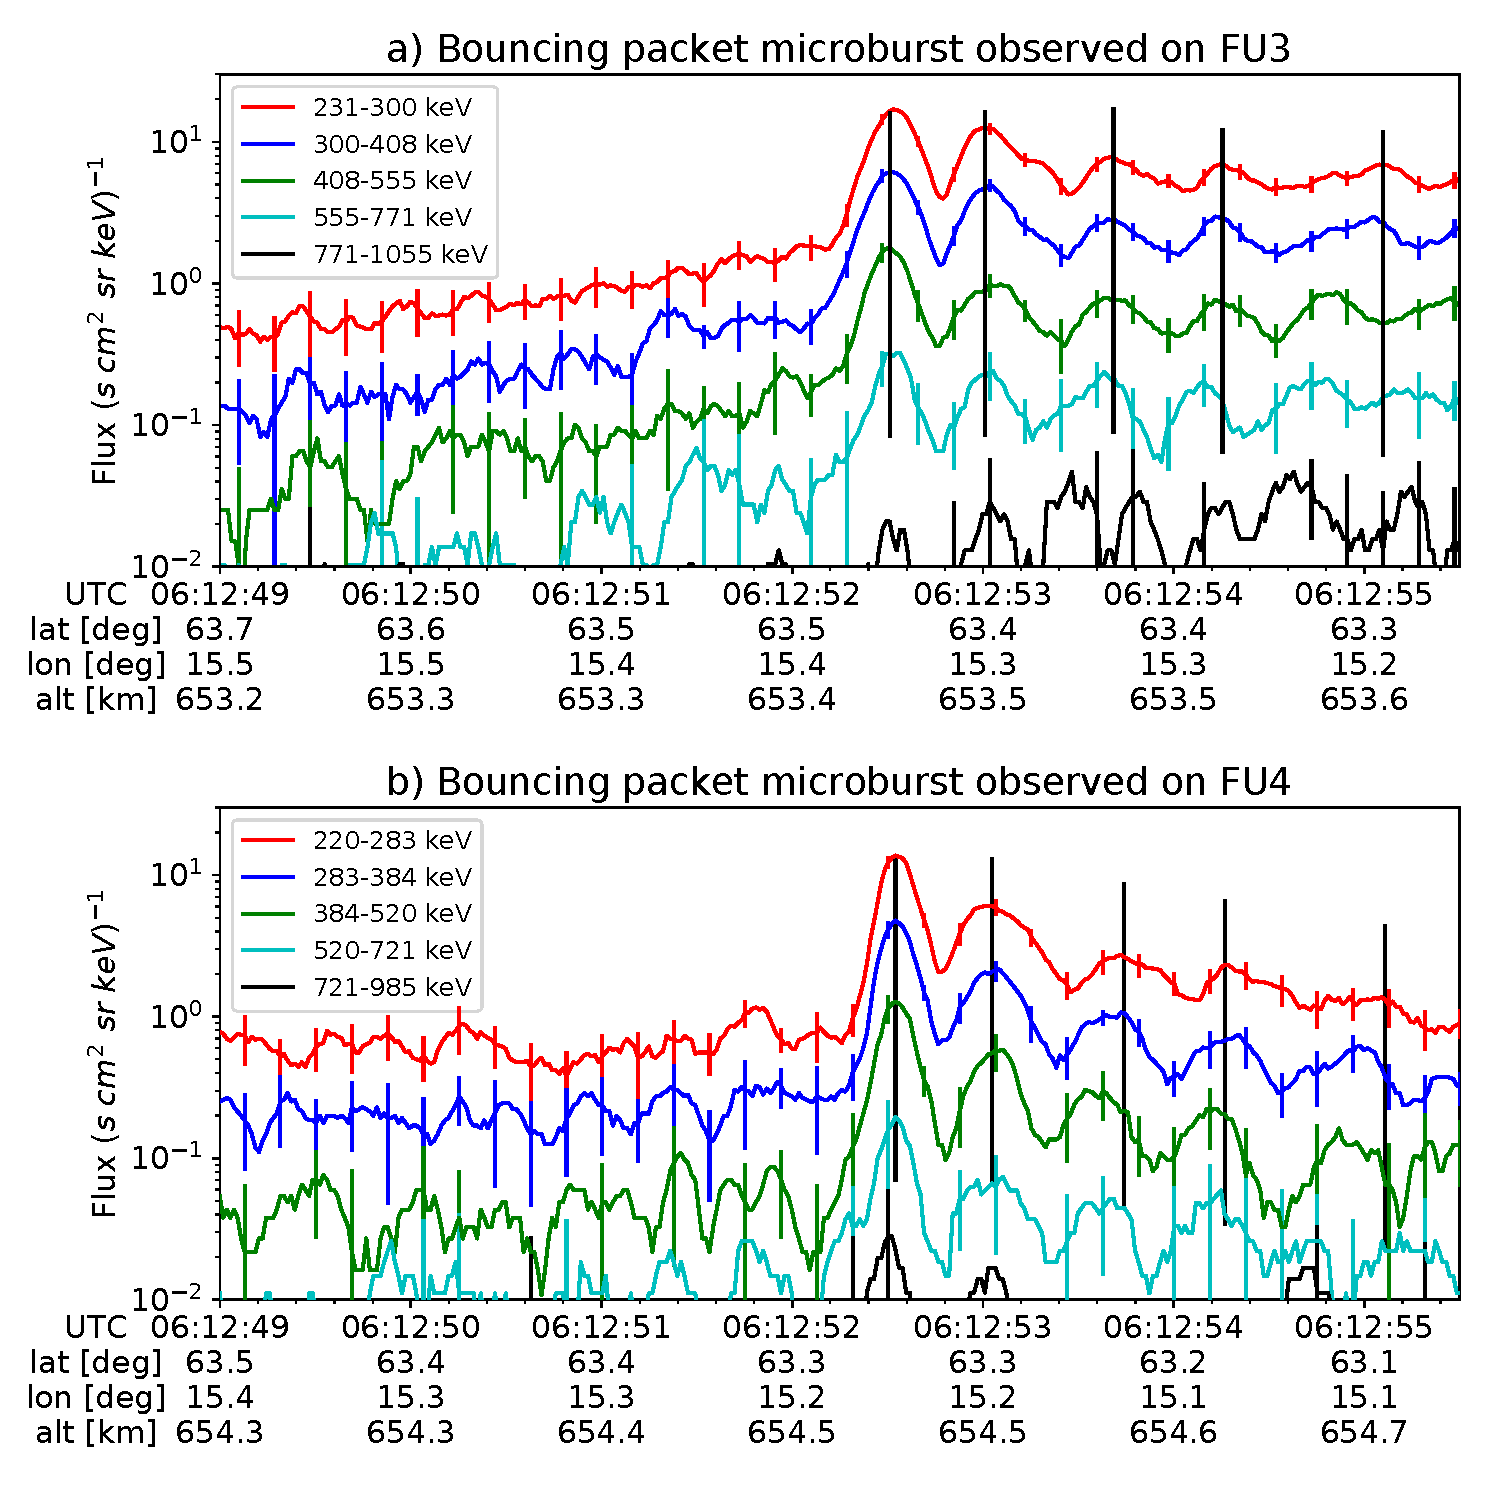
\includegraphics[width=\textwidth]{hires_plot_log_8pt_smooth_pos_v2.pdf}
\caption{HiRes data of the microburst observed at February 2nd, 2015 at 06:12:53 UT, smoothed with a 150 ms rolling average. The subsequent bounces showed some energy dispersion. As discussed in section \ref{analysis} a time correction of -2.28 s was applied to FU3. While the flux from five energy channels is shown, only channels with reasonable counting statistics were used for the spatial scale analysis. Vertical colored bars show the $\sqrt{N}$ error every 10th data point and vertical black bars are lined up with the peaks in the 220-283 keV energy channel to help identify dispersion.}
\label{hires_plot}
\end{figure}

\begin{figure}
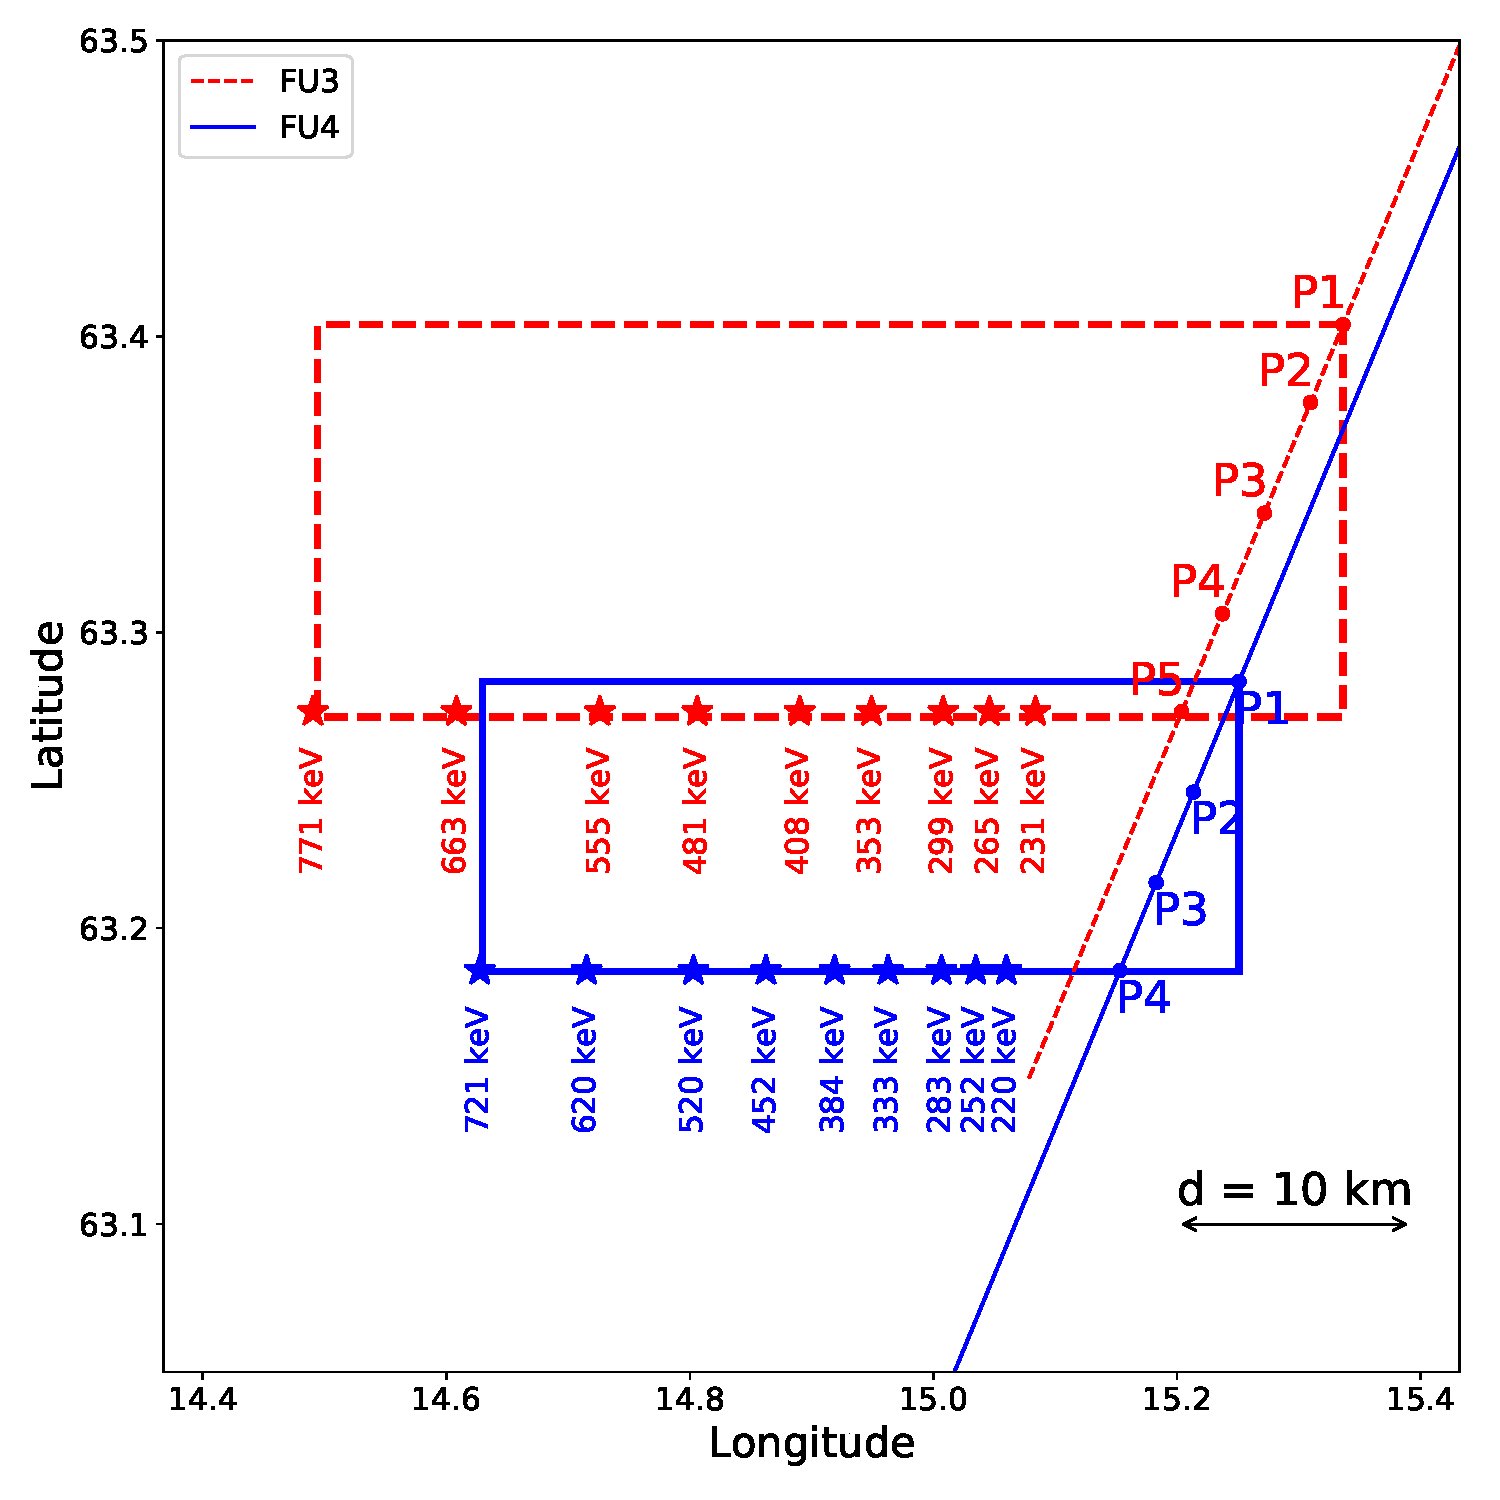
\includegraphics[width=\textwidth]{decay_microburst_distance_corrected_CH4_last_pk_drift_color_2.pdf}
\caption{The topology of the FIREBIRD-II orbit and the multiple bounces of the microburst projected onto latitude and longitude with axis scaled to equal distance. Attributes relating to FU3 shown in red dashed lines, and FU4 with blue solid lines. The spacecraft path is shown with the diagonal lines, starting at the upper right corner. The labels P1-4 for FU4 and P1-5 for FU3 indicate where the spacecraft were when the N$^{th}$ peak was seen in the lowest energy channel in the HiRes data. The stars with the accompanying energy labels represent the locations of the electrons with that energy that started at time of P1, and were seen at the last peak on each spacecraft. The rectangles represent the lower bound of the microburst scale size, assuming that the majority of the electrons were in the upper boundary of energy channel 4.}
\label{map_plot}
\end{figure}

\begin{figure}
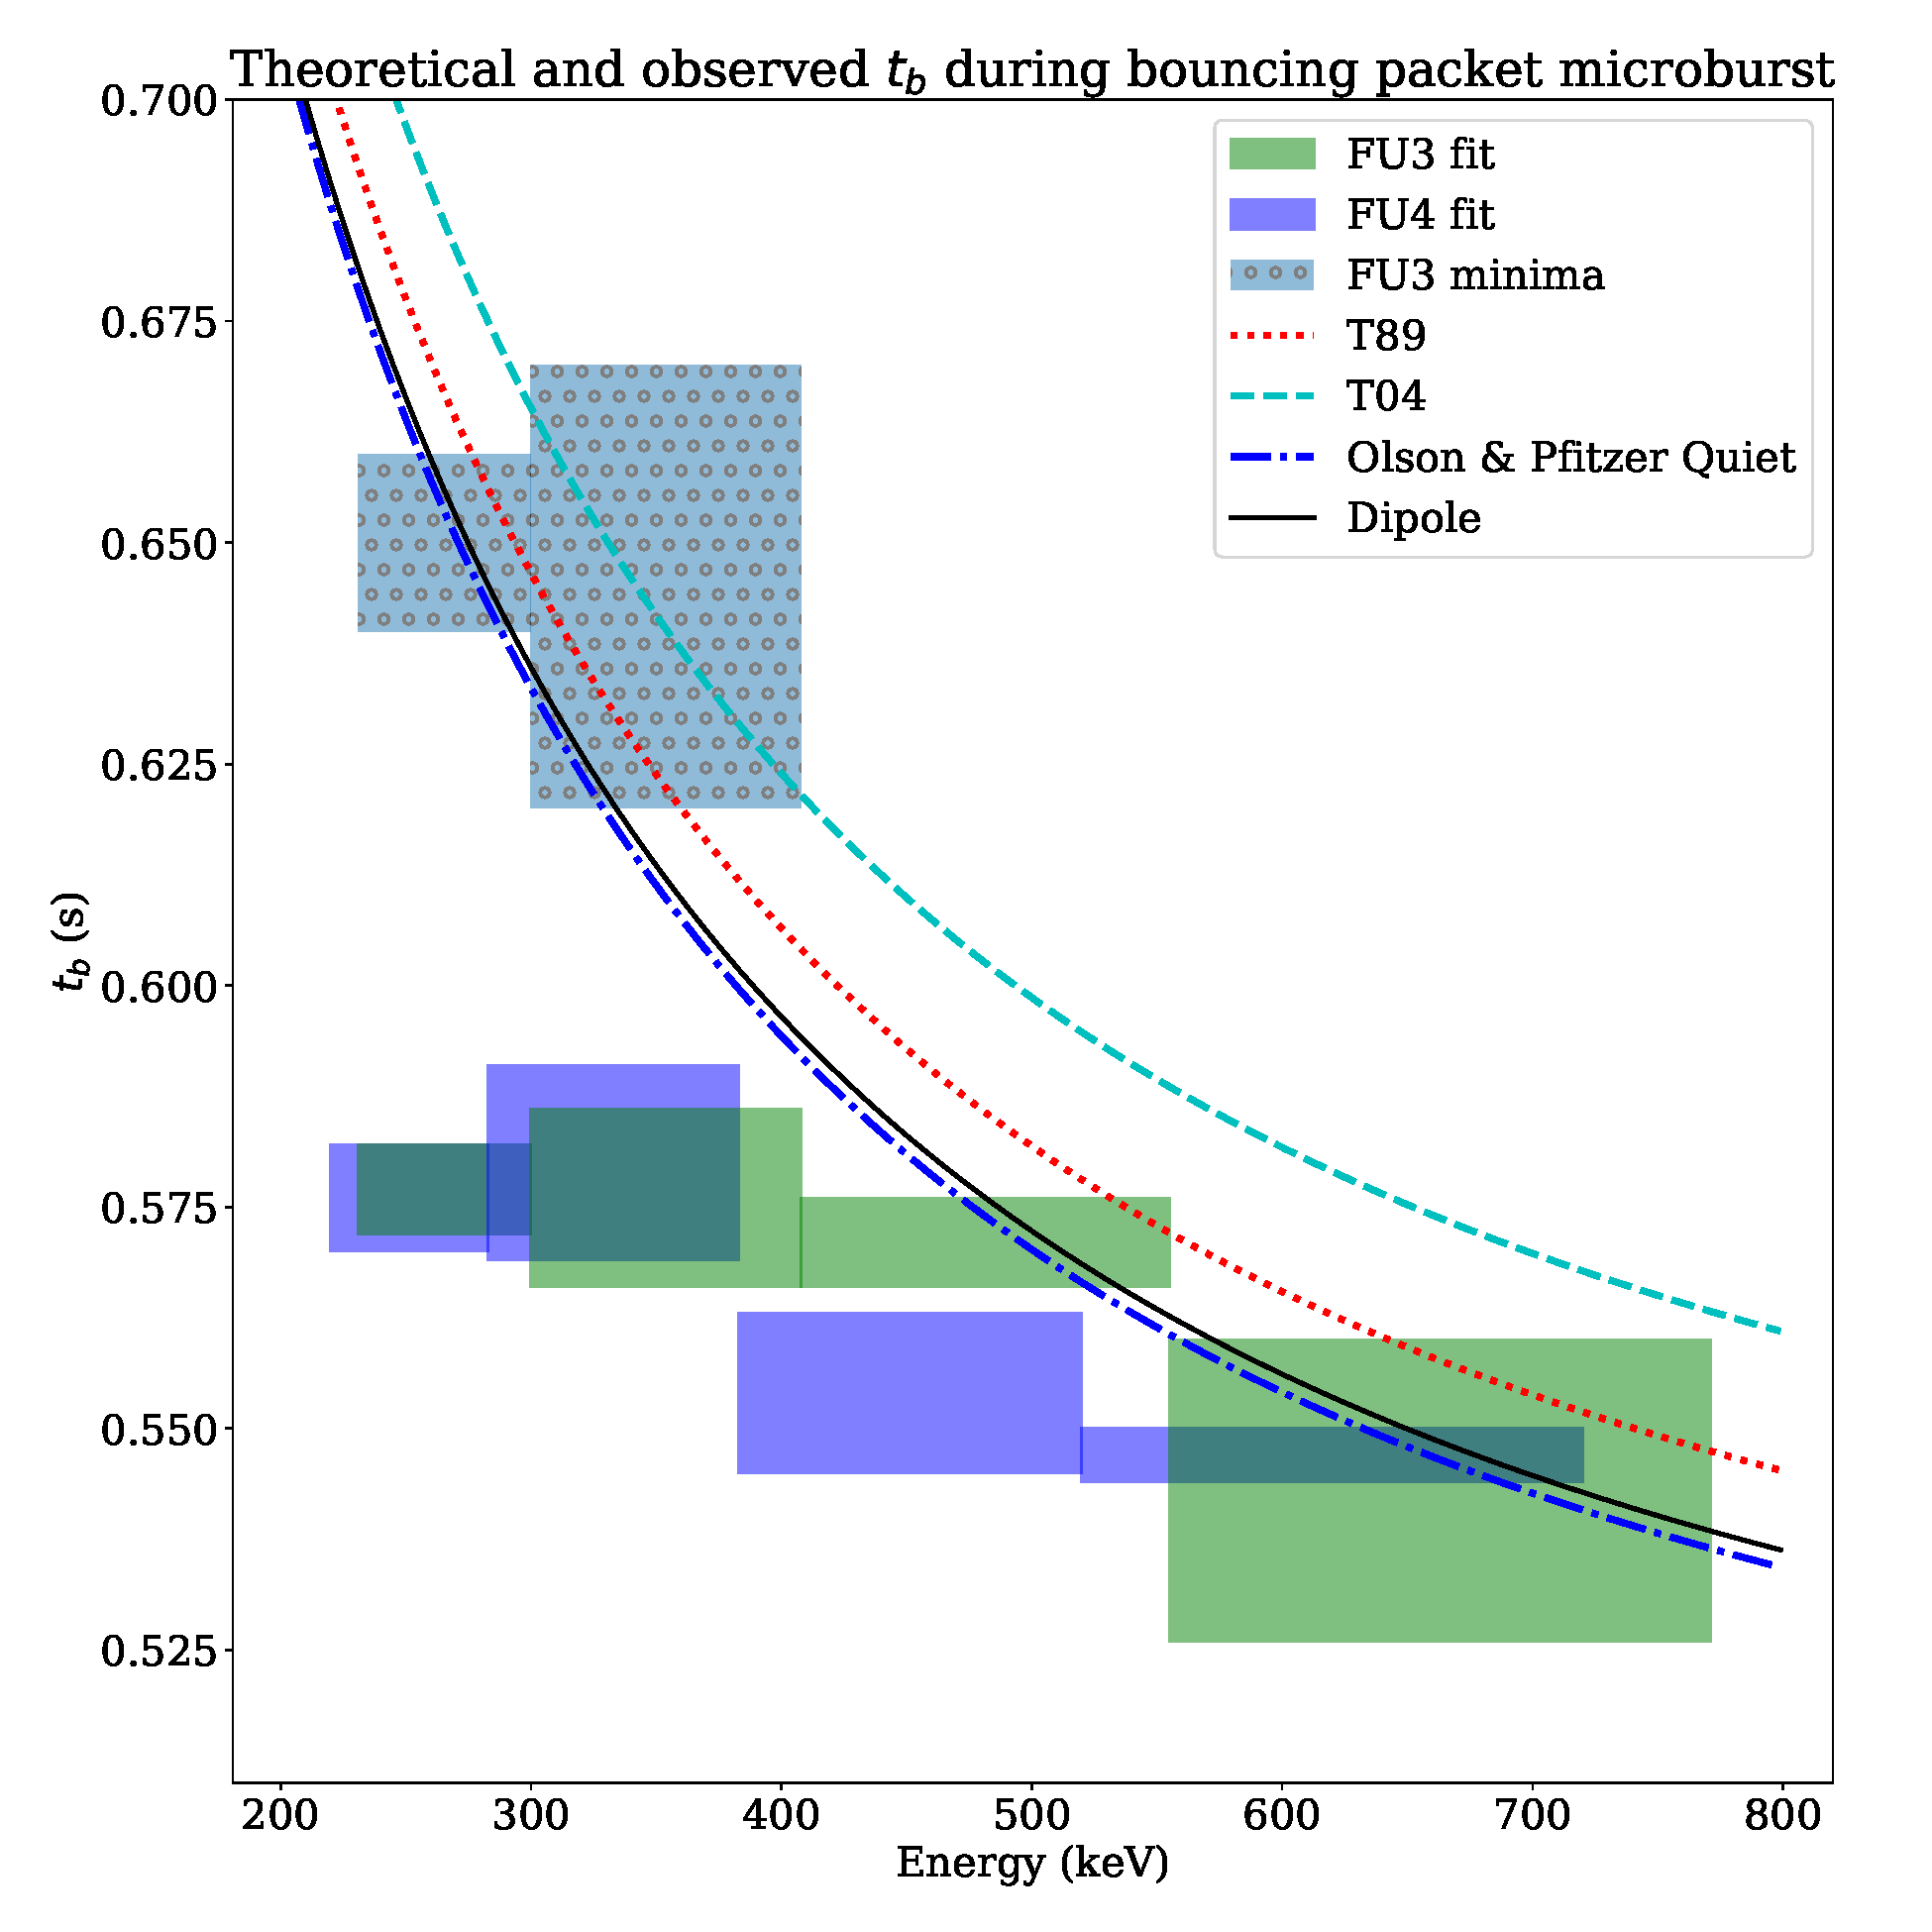
\includegraphics[width=\textwidth]{detrended_bounce_period_boxed_adj.pdf}
\caption{Observed and theoretical $t_b$ for electrons of energies from 200 to 770 keV. The solid black line is $t_b$ in a dipole magnetic field, derived in \citet{Schulz1974}. The red and cyan dashed lines are the $t_b$ derived using the T89, and T04 magnetic field models with IRBEM. Lastly, the blue dashed curve is the $t_b$ derived using the Olson \& Pfitzer Quiet model. The green and purple rectangles represent the observed $t_b$ for FU3 and FU4 using a Gaussian fit, respectively. The blue rectangles represent the observed $t_b$ calculated with the minima between the bounces. The width of the boxes represent the width of those energy channels, and the height represents the uncertainty from the fit.}
\label{tb_plot}
\end{figure}

%% ------------------------------------------------------------------------ %%
%% Citations

% Please use ONLY \citet and \citep for reference citations.
% DO NOT use other cite commands (e.g., \cite, \citeyear, \nocite, \citealp, etc.).


%% Example \citet and \citep:
%  ...as shown by \citet{Boug10}, \citet{Buiz07}, \citet{Fra10},
%  \citet{Ghel00}, and \citet{Leit74}. 

%  ...as shown by \citep{Boug10}, \citep{Buiz07}, \citep{Fra10},
%  \citep{Ghel00, Leit74}. 

%  ...has been shown \citep [e.g.,][]{Boug10,Buiz07,Fra10}.

\bibliography{/home/mike/Dropbox/0_firebird_research/A_presentations/refs}

%%  REFERENCE LIST AND TEXT CITATIONS
%
% Either type in your references using
%
% \begin{thebibliography}{}
% \bibitem[{\textit{Kobayashi et~al.}}(2003)]{R2013} Kobayashi, T.,
% Tran, A.~H., Nishijo, H., Ono, T., and Matsumoto, G.  (2003).
% Contribution of hippocampal place cell activity to learning and
% formation of goal-directed navigation in rats. \textit{Neuroscience}
% 117, 1025--1035.
%
% \bibitem{}
% Text
% \end{thebibliography}
%
%%%%%%%%%%%%%%%%%%%%%%%%%%%%%%%%%%%%%%%%%%%%%%%
% Or, to use BibTeX:
%
% Follow these steps
%
% 1. Type in \bibliography{<name of your .bib file>} 
%    Run LaTeX on your LaTeX file.
%
% 2. Run BiBTeX on your LaTeX file.
%
% 3. Open the new .bbl file containing the reference list and
%   copy all the contents into your LaTeX file here.
%
% 4. Run LaTeX on your new file which will produce the citations.
%
% AGU does not want a .bib or a .bbl file. Please copy in the contents of your .bbl file here.


%% After you run BibTeX, Copy in the contents of the .bbl file here:
%\begin{thebibliography}{35}
%\end{thebibliography}

%%%%%%%%%%%%%%%%%%%%%%%%%%%%%%%%%%%%%%%%%%%%%%%%%%%%%%%%%%%%%%%%%%%%%
% Track Changes:
% To add words, \added{<word added>}
% To delete words, \deleted{<word deleted>}
% To replace words, \replace{<word to be replaced>}{<replacement word>}
% To explain why change was made: \explain{<explanation>} This will put
% a comment into the right margin.

%%%%%%%%%%%%%%%%%%%%%%%%%%%%%%%%%%%%%%%%%%%%%%%%%%%%%%%%%%%%%%%%%%%%%
% At the end of the document, use \listofchanges, which will list the
% changes and the page and line number where the change was made.

% When final version, \listofchanges will not produce anything,
% \added{<word or words>} word will be printed, \deleted{<word or words} will take away the word,
% \replaced{<delete this word>}{<replace with this word>} will print only the replacement word.
%  In the final version, \explain will not print anything.
%%%%%%%%%%%%%%%%%%%%%%%%%%%%%%%%%%%%%%%%%%%%%%%%%%%%%%%%%%%%%%%%%%%%%

%%%
%\listofchanges
%%%

\end{document}

%%%%%%%%%%%%%%%%%%%%%%%%%%%%%%%%%%%%%
%% Supporting Information
%% (Optional) See AGUSuppInfoSamp.tex/pdf for requirements 
%% for Supporting Information.
%%%%%%%%%%%%%%%%%%%%%%%%%%%%%%%%%%%%%



%%%%%%%%%%%%%%%%%%%%%%%%%%%%%%%%%%%%%%%%%%%%%%%%%%%%%%%%%%%%%%%

More Information and Advice:

%% ------------------------------------------------------------------------ %%
%
%  SECTION HEADS
%
%% ------------------------------------------------------------------------ %%

% Capitalize the first letter of each word (except for
% prepositions, conjunctions, and articles that are
% three or fewer letters).

% AGU follows standard outline style; therefore, there cannot be a section 1 without
% a section 2, or a section 2.3.1 without a section 2.3.2.
% Please make sure your section numbers are balanced.
% ---------------
% Level 1 head
%
% Use the \section{} command to identify level 1 heads;
% type the appropriate head wording between the curly
% brackets, as shown below.
%
%An example:
%\section{Level 1 Head: Introduction}
%
% ---------------
% Level 2 head
%
% Use the \subsection{} command to identify level 2 heads.
%An example:
%\subsection{Level 2 Head}
%
% ---------------
% Level 3 head
%
% Use the \subsubsection{} command to identify level 3 heads
%An example:
%\subsubsection{Level 3 Head}
%
%---------------
% Level 4 head
%
% Use the \subsubsubsection{} command to identify level 3 heads
% An example:
%\subsubsubsection{Level 4 Head} An example.
%
%% ------------------------------------------------------------------------ %%
%
%  IN-TEXT LISTS
%
%% ------------------------------------------------------------------------ %%
%
% Do not use bulleted lists; enumerated lists are okay.
% \begin{enumerate}
% \item
% \item
% \item
% \end{enumerate}
%
%% ------------------------------------------------------------------------ %%
%
%  EQUATIONS
%
%% ------------------------------------------------------------------------ %%

% Single-line equations are centered.
% Equation arrays will appear left-aligned.

Math coded inside display math mode \[ ...\]
 will not be numbered, e.g.,:
 \[ x^2=y^2 + z^2\]

 Math coded inside \begin{equation} and \end{equation} will
 be automatically numbered, e.g.,:
 \begin{equation}
 x^2=y^2 + z^2
 \end{equation}


% To create multiline equations, use the
% \begin{eqnarray} and \end{eqnarray} environment
% as demonstrated below.
\begin{eqnarray}
  x_{1} & = & (x - x_{0}) \cos \Theta \nonumber \\
        && + (y - y_{0}) \sin \Theta  \nonumber \\
  y_{1} & = & -(x - x_{0}) \sin \Theta \nonumber \\
        && + (y - y_{0}) \cos \Theta.
\end{eqnarray}

%If you don't want an equation number, use the star form:
%\begin{eqnarray*}...\end{eqnarray*}

% Break each line at a sign of operation
% (+, -, etc.) if possible, with the sign of operation
% on the new line.

% Indent second and subsequent lines to align with
% the first character following the equal sign on the
% first line.

% Use an \hspace{} command to insert horizontal space
% into your equation if necessary. Place an appropriate
% unit of measure between the curly braces, e.g.
% \hspace{1in}; you may have to experiment to achieve
% the correct amount of space.


%% ------------------------------------------------------------------------ %%
%
%  EQUATION NUMBERING: COUNTER
%
%% ------------------------------------------------------------------------ %%

% You may change equation numbering by resetting
% the equation counter or by explicitly numbering
% an equation.

% To explicitly number an equation, type \eqnum{}
% (with the desired number between the brackets)
% after the \begin{equation} or \begin{eqnarray}
% command.  The \eqnum{} command will affect only
% the equation it appears with; LaTeX will number
% any equations appearing later in the manuscript
% according to the equation counter.
%

% If you have a multiline equation that needs only
% one equation number, use a \nonumber command in
% front of the double backslashes (\\) as shown in
% the multiline equation above.

% If you are using line numbers, remember to surround
% equations with \begin{linenomath*}...\end{linenomath*}

%  To add line numbers to lines in equations:
%  \begin{linenomath*}
%  \begin{equation}
%  \end{equation}
%  \end{linenomath*}



